\documentclass{article}
\usepackage[margin=.5in]{geometry}
\usepackage{graphicx, dblfloatfix}
\usepackage{amsmath, amssymb, amsfonts, mathrsfs, mathtools, physics}
\usepackage[english]{babel}
\usepackage[autostyle, english = american]{csquotes}
\usepackage[normalem]{ulem}
\usepackage[title,titletoc,toc]{appendix}
\usepackage{pgfplotstable}
\usepackage{array, booktabs, colortbl}
\MakeOuterQuote{"}

\pgfplotsset{compat=1.12}


\newcommand{\redchi}{$\tilde{\chi}^2\,$}
\DeclareMathOperator{\cov}{cov}
\DeclarePairedDelimiter{\parens}{\lparen}{\rparen}

\title{Neutron Studies}
\author{Aman LaChapelle}

\begin{document}
\raggedright
\maketitle

\begin{abstract}
  Here we show a method by which we can measure an effective radius for the neutron, as well as observe the reaction that creates a deuteron.  We demonstrate techniques which can be used in order to perform these measurements using fast neutrons emitted from a PuBe source.
\end{abstract}

\tableofcontents
\newpage

\section{Introduction}
  In this experiment we demonstrate means by which we are able to observe the reaction that creates a deuteron, as well as measuring the size of the neutron.  We collect data for multiple thicknesses of each absorber in order to determine the scattering cross-section of the fast neutrons as they pass through the absorbers.  Based on the intensity of neutrons that hit the plastic scintillator detector, we are able to determine how many were absorbed or back-scattered.  From this intensity, we are able to calculate the size of the nucleus since neutrons will scatter only if they pass within about one wavelength (the neutron's de Broglie wavelength) of the nucleus.  Thus, based on the proportion of neutrons that pass through the absorber we will be able to determine an approximate density (and thus size) for the nuclei of that absorber.

\section{Theory}
  \subsection{Deuteron Production}
  There is a stable bound state of a proton and a neutron called a deuteron.  In general, if the neutron has energy comparable to the proton, it will be possible to have the neutron hit the proton and create this bound state.  It differs from deuterium in that it does not necessarily have the bound electron that a hydrogen atom typically does.  The important concept to note is that the deuteron is a bound state of a neutron and of a proton.  This state has lower energy than the sum of the incoming energy of the neutron and proton, and so the reaction that creates a deuteron is characterized by a capture photon on the order of 2 MeV.  Since the neutrons and protons that have low enough energy to fall into a bound state like this one are generally barely moving if at all, we take their energy to be roughly equal to their rest mass for the purposes of a rough calculation.  Use the following reaction:
  \begin{equation*}
    n + p \rightarrow d + \gamma
  \end{equation*}
  We determine that given the rest energy of the neutron, proton, and deuteron, the capture photon should have an energy of around 2.1 MeV.

  \hspace{.25cm}

  Experimentally, this reaction is not particularly simple to measure.  However, we take a hydrogen-rich substance - paraffin - and place it in the path of the fast neutrons.  We then place that in front of our detector which we expect to measure the capture photons.  However, there is a lot of ambient energy, which translates into a lot of ambient photons.  This translates into, experimentally, shielding the detector with lead bricks in order to attenuate photons coming from the paraffin surrounding the PuBe core, or even ambient lighting, for example.  Thus we take a series of spectra to determine background rates, and we will perform a check to make sure that the deuteron production is actually occurring with the hydrogen atoms in the paraffin and not (for example) the creation and decay of Carbon-13.

  \subsection{Neutron Cross-Section/Nucleus Size}
  Neutrons typically interact with low-Z materials - that is, they interact with materials that have a comparable atomic size/mass to the neutron.  Carbon is heavier, but only by an order of magnitude.  What this means is that carbon is a good attenuator of these fast neutrons.  What it will not do, however, is to give off the capture photons that we got used to in the first part of the experiment, as will happen when the neutron interacts with a hydrogen nucleus to create a deuteron.  Thus, in order to measure the attenuation rate of neutrons due to different materials (in order to determine a cross-section), we will have to look at continuous data.  We fit our PMT with a plastic scintillator.  The incoming fast neutrons will scatter the hydrogen atoms in the plastic and cause light emission.  These light emissions are seen by the PMT and translated into voltage pulses that allow us to measure the energy deposited by the scattered protons (and thus, roughly, the incoming neutrons).

  \hspace{.25cm}

  The detector is sensitive to incoming photons as well, however, its response is different, which allows us to find an effective region of interest for which the response is due to protons and not to incident photons.  In Figure~\ref{response} we can see that the response for a 7 MeV proton is roughly 3 times the response of a 1.275 MeV photon.  Since we have access to Na-22 sources which emit 1.275 MeV photons as one of their full energy peaks, we are able to perform a sort of calibration on the axis and roughly determine a region of interest by looking for the Compton edges on the Na-22 spectrum and using a ROI that begins at roughly 3 times the 1.275 MeV Compton edge and goes to the end of the detector range, as we can see in Figure~\ref{roi}.

  \hspace{.25cm}

  We can perform a rough calculation in determining the region of interest if we consider the Compton edge.  Given the Compton formula,

  \begin{equation*}
    E' = \frac{E}{1+\frac{E}{mc^2}\parens*{1-\cos{\theta}}}
  \end{equation*}

  and given that the scattering angle is going to be roughly $\pi$, we can therefore calculate an approximate energy for the scattered photon $E'$ given input energies.  If we calculate $E'$ for a proton of energy that is approximately 7 MeV and for an electron of 1 MeV, and take the quotient, we return a value of approximately 3, as we can read from Figure~\ref{response}. Thus we can be certain we will set our ROI to begin at the channel that is 3 times the Na-22 1275 keV Compton edge.

  \hspace{.25cm}

  In actually collecting data, we shield the detector with approximately 4 inches of lead in order to attenuate any photons that are coming either from the paraffin shield around the PuBe source or any other sources in the room.  We are interested in the count rate of neutrons as they pass through various absorbers, and as such we are \textbf{not} interested in the counts that we gain from other, ambient sources.  In this spirit, we measure the ambient background by blocking the detector from the source with approx. 28 inches of Pb.  We can then integrate the region of interest for each absorber element and thickness in order to determine a cross section for the absorbers.  From this, we will be able to calculate an effective radius for the neutron.

  \hspace{.25cm}

  The Ramsauer model suggests that nuclei present a cross section that is equal to twice their effective area.  That is,
  \begin{equation*}
    \sigma = 2\pi\parens*{R + \lambda}^2
  \end{equation*}
  where $R$ is the radius, and $\lambda$ is the deBroglie wavelength of the neutron.  According to this model, scattering only occurs if the neutron passes within about 1 wavelength of the nucleus.  This means that the radius of the nucleus roughly obeys the rule
  \begin{equation*}
    R = r_0A^{1/3}
  \end{equation*}
  which implies that
  \begin{equation*}
    \sqrt{\frac{\sigma}{2\pi}} = r_0 A^{1/3} + \lambda
  \end{equation*}
  where $r_0$ is the radius of the neutron and $A$ is the average atomic mass.  We should thus be able to, given accurate cross sections, determine the radius of the neutron by plotting $\sqrt{\frac{\sigma}{2\pi}}$ versus $A^{1/3}$, fitting a line and extracting the slope and intercept of that line.  Those two parameters should return the radius and the deBroglie wavelength of a neutron, respectively.

\section{Experimental Procedure}
  \subsection{Neutron Mass}
  stuff about the deuteron reaction here, we use the energy of the capture photon to get the mass of the neutron

  \subsection{Neutron Radius}
  stuff about how we used the cross sections and integrated to get the count rates and fit exponentials and whatnot

  \hspace{.25cm}

  merge with data/analysis maybe?  Or merge with the theory section?


\section{Data and Uncertainty Analysis}

\section{Conclusion}

\section{Figures}
  \begin{figure}[!htb]
    \centering
    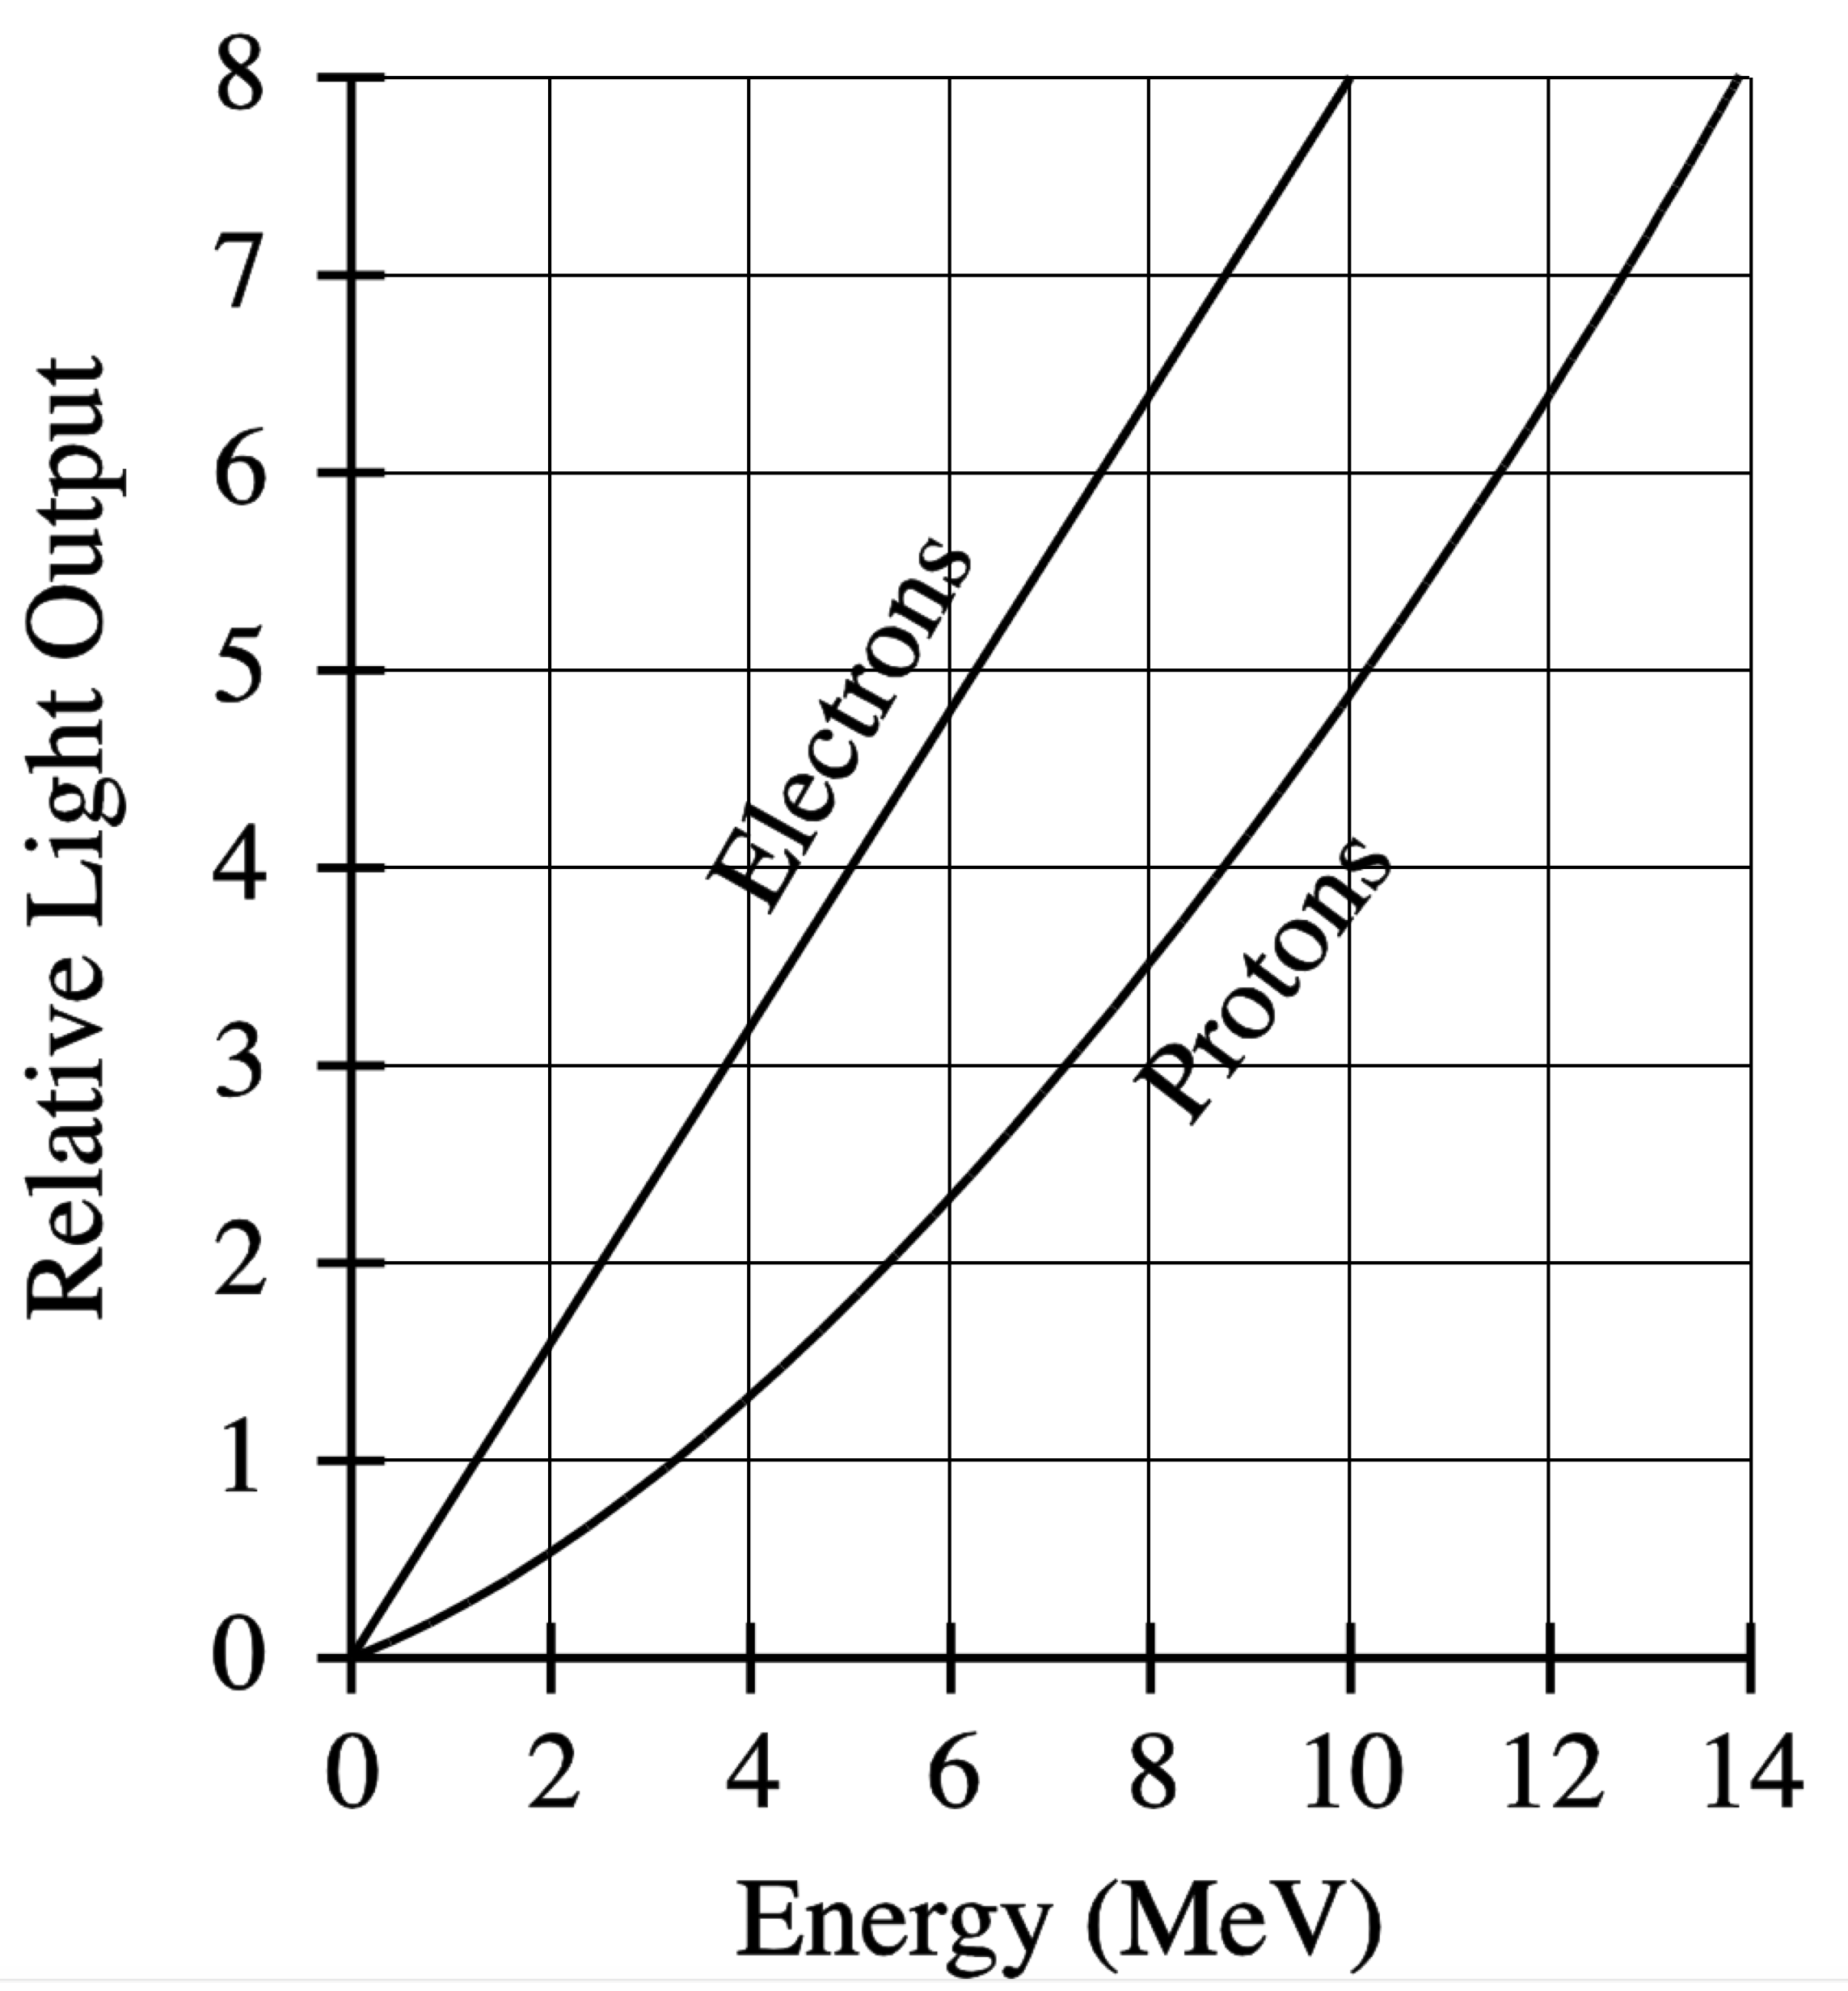
\includegraphics[scale=.5]{relative_response.png}
    \caption{Relative light output resulting from incident photons - which scatter electrons, and from incident neutrons which scatter protons.}
    \label{response}
  \end{figure}

  \hspace{.25cm}

  \begin{figure}[!htb]
    \centering
    \begin{tabular}{c c}
      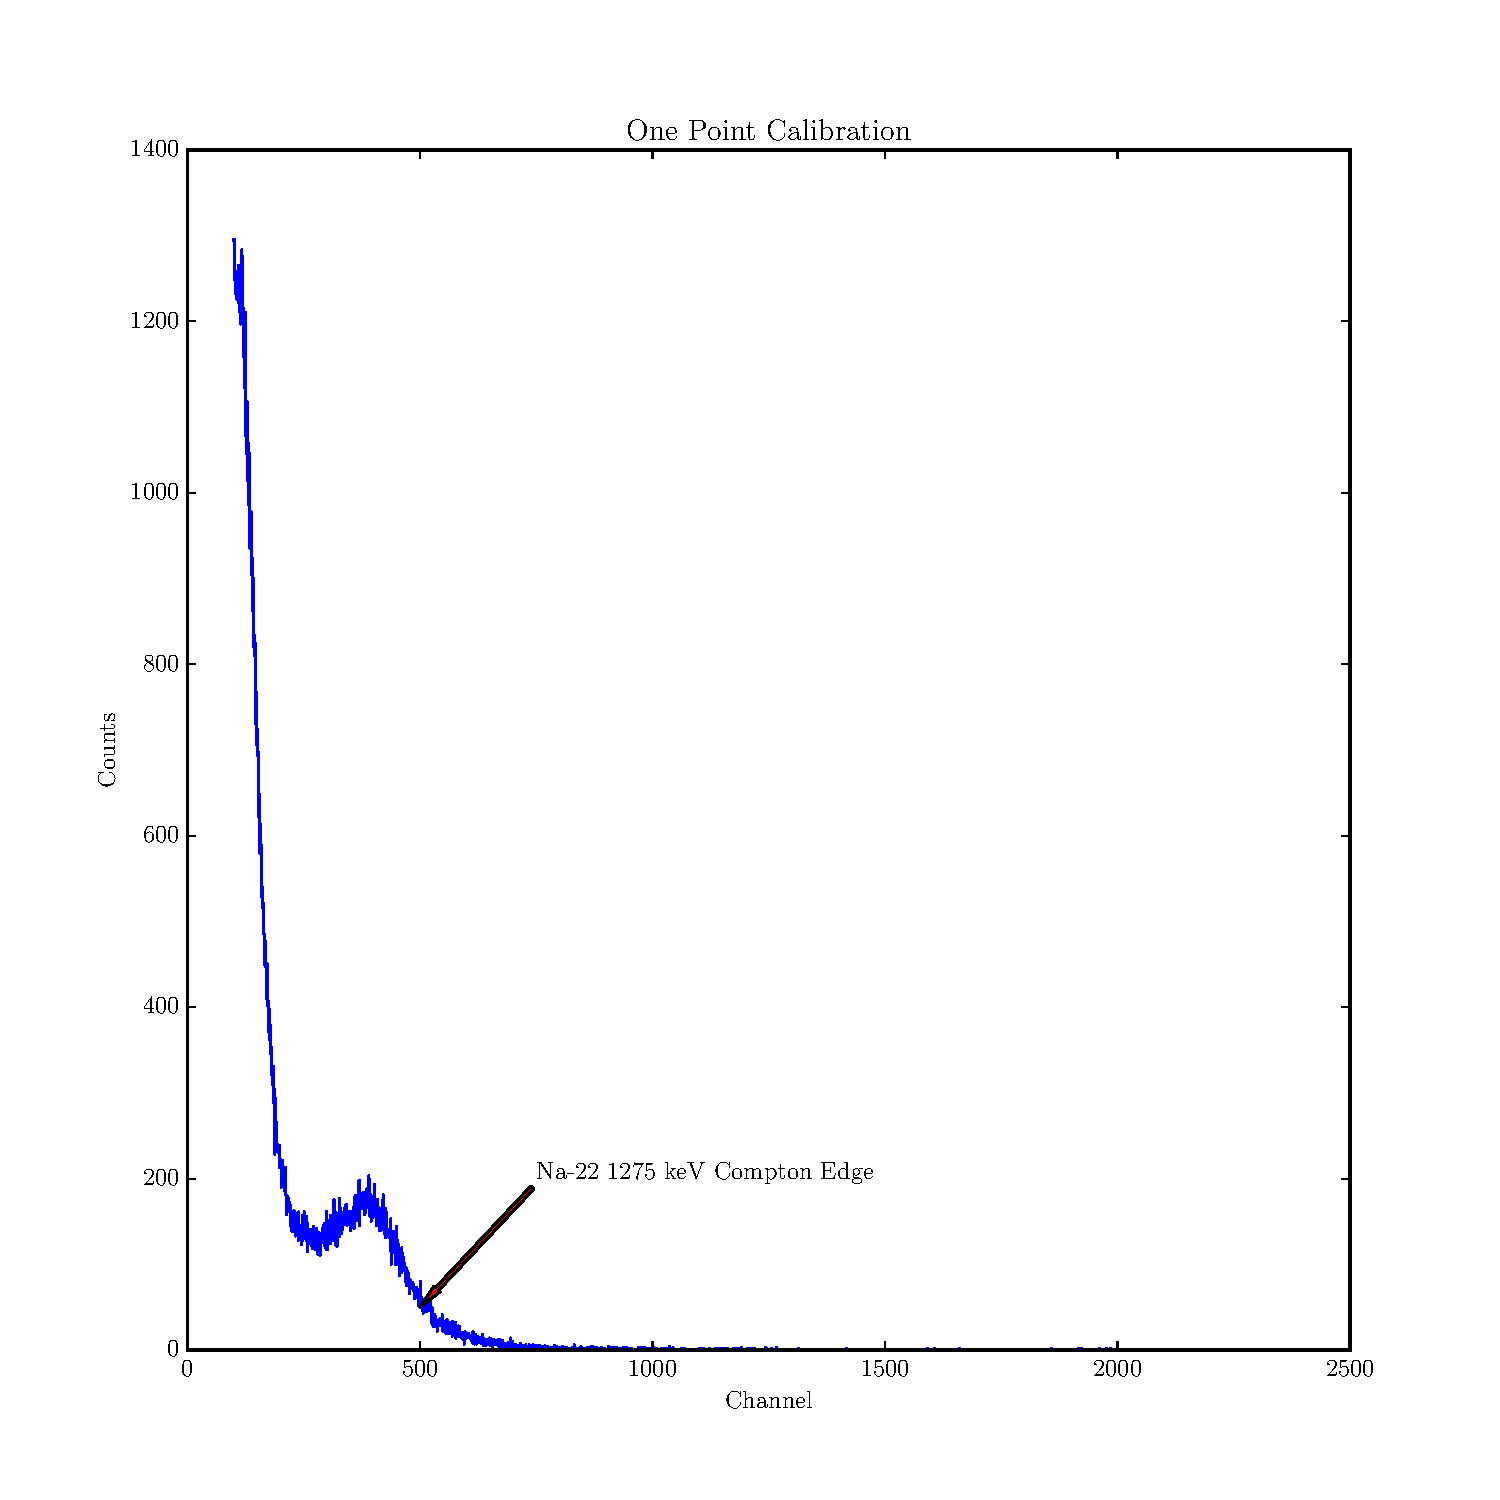
\includegraphics[scale=.4]{../plots/na_calibration_absorber_countrates.pdf} \\ 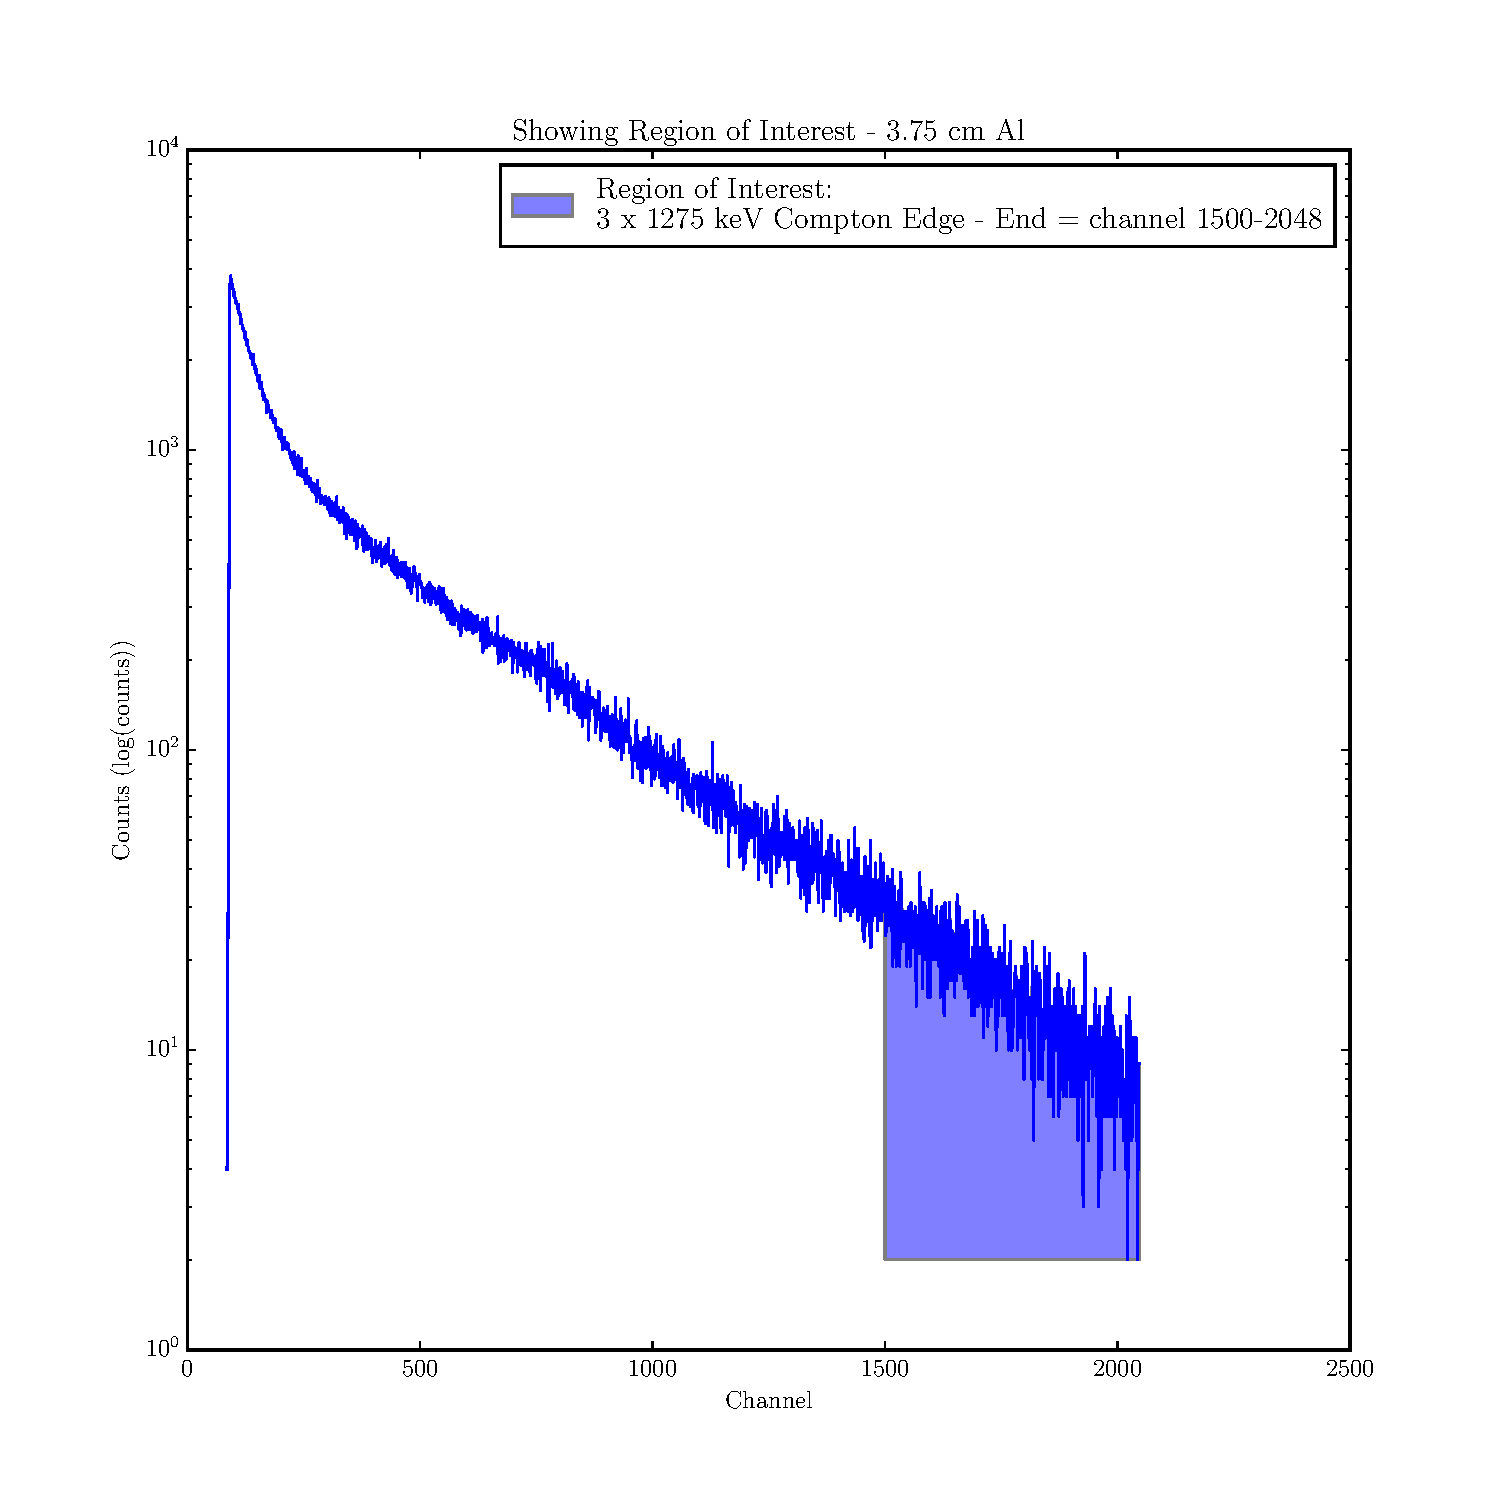
\includegraphics[scale=.4]{../plots/example_cross_section_highlight_roi.pdf}
    \end{tabular}
    \caption{Since the 1275 keV Compton edge is a rather broad feature, we choose one end, and a round number to make further calculations nicer.  Especially since the channels are integers, we cannot subdivide them and it is therefore beneficial to choose a nice round number that has a multiple of 3 in the integers.  Note that the plot that highlights the ROI is a semi-log plot in y so that we can better see the region of interest - as we can see from the Na-22 spectrum, one end tends to dominate if we don't show the counts axis in log scale.}
    \label{roi}
  \end{figure}

  \begin{figure}[!htb]
    \centering
    \begin{tabular}{c c}
      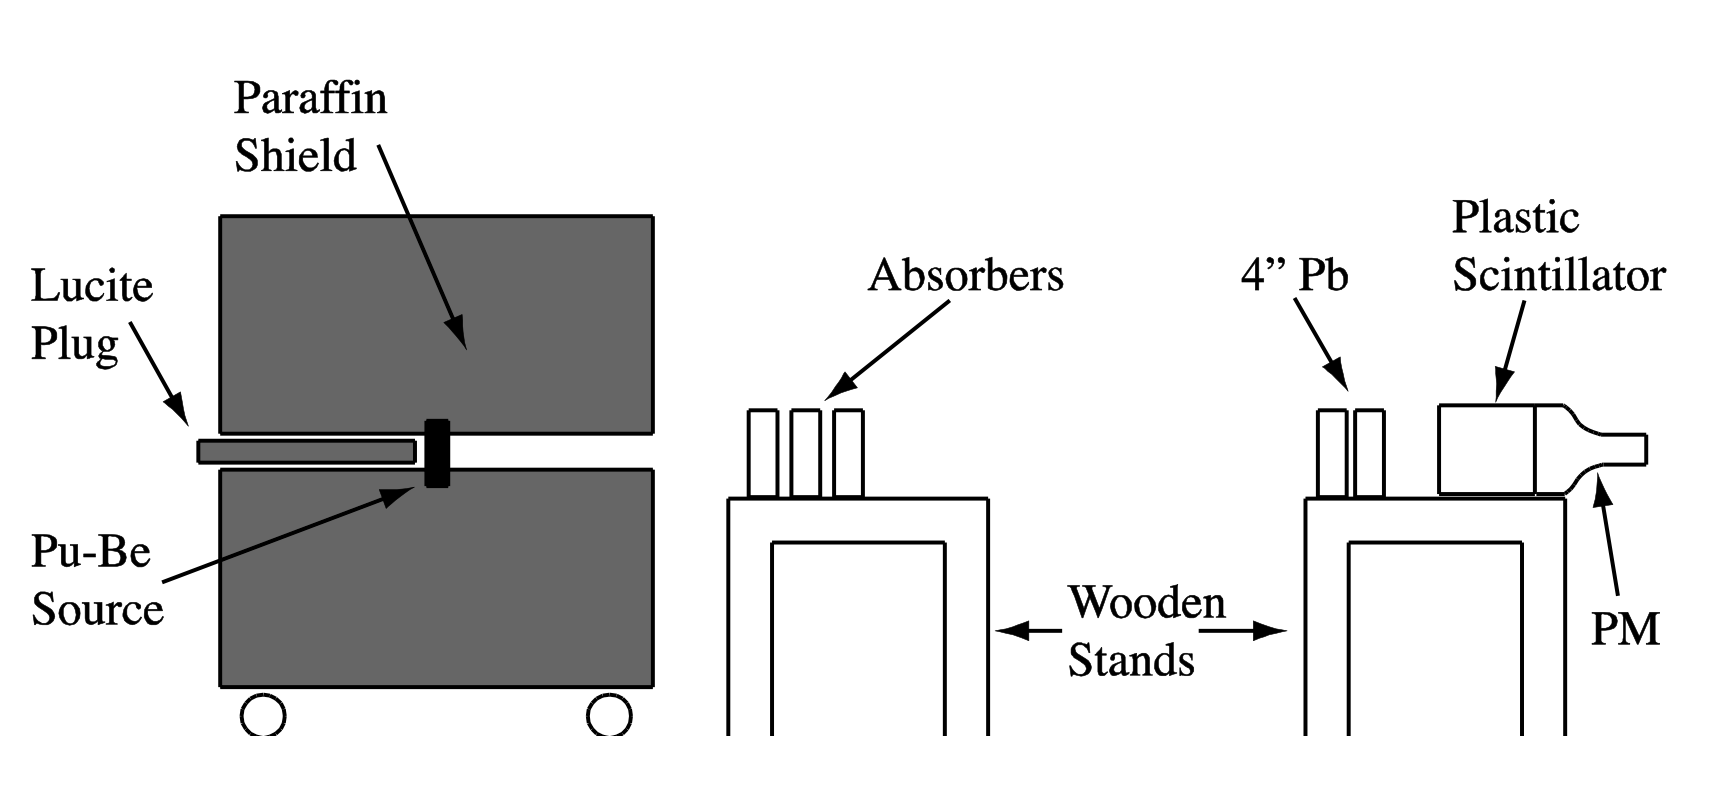
\includegraphics[scale=.25]{cross_section_apparatus.png} \\ 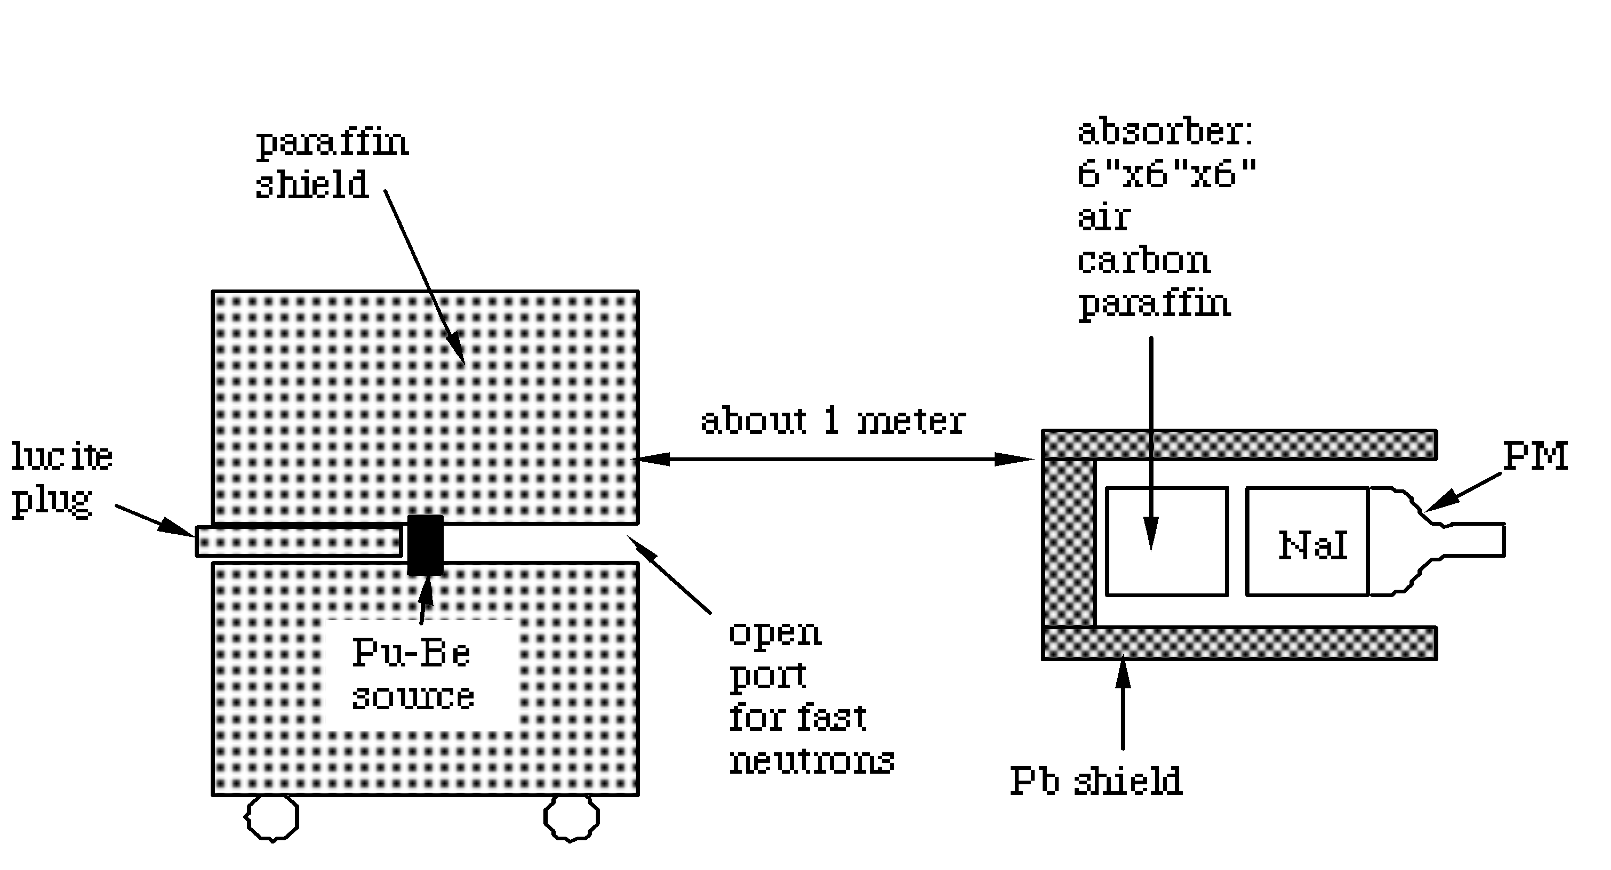
\includegraphics[scale=.25]{day_1_apparatus.png} \\
    \end{tabular}
    \caption{The top image is the experimental setup that we used to determine the radius of the neutron, the bottom image is the setup that allowed us to measure the capture photons from the deuteron reaction.  In reality, the wooden stand for the absorber was much closer to the detector for practicality reasons, but the essential setup is the same.}
    \label{apparatus}
  \end{figure}

\end{document}
